\section{Case study: Berry (1994) and the mean-utility method}\label{sec:07-berry}

The estimating equations of \cref{sec:07-inversion,sec:07-endogeneity,sec:07-supply,sec:07-nested} go back to
one article, \citet{Berry1994}. This section reads it in its own terms. We cite its equation numbers so that a
reader can follow the original, and we point back to the sections above for derivations already given. Page
numbers refer to the journal pagination.

\subsection{The question}\label{sec:07-berry-question}

Berry asks how to estimate demand and cost from a cross section of oligopoly markets with differentiated
products, when prices are correlated with demand factors that the econometrician does not observe. In
homogeneous-goods markets the demand error has long been read as unobserved demand factors, which the supply
relation shows to be correlated with price. Ignoring that correlation produces upward-sloping demand curves and
similar anomalies (p.~243). Berry argues that differentiated products raise the same problem whenever some
characteristics are unobserved, and that unobserved characteristics are common. Style is hard to quantify. Physically similar
products differ in perceived quality, durability, status or service. The relevant characteristics may outnumber
the observations.

Instrumental variables fix the problem for a homogeneous good. In a discrete-choice model, however, price and the
unobserved characteristic both enter the share equation nonlinearly, which blocks a direct application. The
alternatives of the time, reviewed in \cref{sec:07-inversion-problem}, were unattractive. A constant-elasticity
system (Berry's equation (1)) is linear, but $N$ goods bring $N^2$ elasticities, and restricting them a priori is
arbitrary. Discrete choice models without unobserved characteristics produce anomalies such as the
upward-sloping demand for CT scanners in \citet{Trajtenberg1989}. Berry derives demand from a utility model with
few parameters and finds a way to keep instrumental variables. The article is methodological. Its evidence is a
set of Monte Carlo experiments (\cref{sec:07-berry-mc}).

\subsection{The model}\label{sec:07-berry-model}

There are $R$ independent markets. Market $r$ has $N_r$ firms, each selling one product. Product $j$ has observed
characteristics $z_j = (x_j, w_j)$, where $x_j$ shifts demand and $w_j$ shifts marginal cost, an unobserved
demand characteristic $\xi_j$ and an unobserved cost shock $\omega_j$. Firms and consumers observe everything.
The econometrician observes prices, quantities and $z = (z_1, \dots, z_N)$.

\begin{assumption}[Exogenous characteristics]\label{asm:07-berry-exog}
In each market $(\xi_j, \omega_j)_{j=1}^N$ is mean independent of $z$, and markets are independent.
\end{assumption}

Berry himself calls this assumption ``unreasonable in many cases'' (p.~245). Utility is
\begin{equation}\label{eq:07-berry-utility}
u_{ij} = x_j\beta_i - \alpha p_j + \xi_j + \epsilon_{ij} = \delta_j + \mu_{ij} + \epsilon_{ij},
\qquad
\delta_j = x_j\beta - \alpha p_j + \xi_j ,
\end{equation}
with random coefficients $\beta_{ik} = \beta_k + \sigma_k\nu_{ik}$ and $\mu_{ij} = \sum_k x_{jk}\sigma_k\nu_{ik}$
(Berry's equations (2) to (5)). Berry writes $\tilde\beta_i$ and $\zeta_{ik}$ where we write $\beta_i$ and
$\nu_{ik}$, and he calls the composite deviation $v_{ij} = \mu_{ij} + \epsilon_{ij}$ by the name $\nu_{ij}$. The
mean utility $\delta_j$ collects everything common to all consumers.

\begin{remark}[What an i.i.d. shock restricts]\label{rem:07-berry-iid}
Let $\mu_{ij} = 0$, so that tastes vary only through a shock $\epsilon_{ij}$ that is i.i.d. across consumers and
products, with any continuous distribution. Then $s_j = s_j(\boldsymbol\delta)$, and since $p_k$ enters only
$\delta_k$, $\frac{\partial s_j}{\partial p_k} = -\alpha\frac{\partial s_j}{\partial\delta_k}$. Shares determine
$\boldsymbol\delta$ uniquely (\cref{prop:07-invertibility}), so products $j$ and $j'$ with equal shares have equal
mean utilities. Exchangeable shocks then give $\frac{\partial s_j}{\partial\delta_k} = \frac{\partial
s_{j'}}{\partial\delta_k}$, so $j$ and $j'$ have the same cross elasticity with respect to any third price
$p_k$. This holds whether $j$ and $j'$ are two subcompacts or a subcompact and a luxury car (p.~246). The
restriction comes from the i.i.d. additive error alone, so an i.i.d. probit shares it \citep{HausmanWise1978}.
Random coefficients remove it, because those who leave $j$ after a price rise have tastes $\beta_i$ that favor
products resembling $j$.
\end{remark}

Each consumer buys one unit of the best alternative. With $f(\cdot \mid x, \sigma)$ the density of
$\boldsymbol v_i$ and $A_j(\boldsymbol\delta) = \{\boldsymbol v_i : \delta_j + v_{ij} > \delta_k + v_{ik}\ \forall
k \ne j\}$, the share is $s_j = \int_{A_j(\boldsymbol\delta)} f(\boldsymbol v \mid x, \sigma)\,\dd\boldsymbol v$
(equation (6)), and quantity is $q_j = Ms_j$ (equation (7)). With finitely many consumers, observed shares
would carry sampling error of variance $\frac{s_j(1-s_j)}{M}$ (footnote 4), so Berry assumes a continuum. An
outside good, whose price does not respond to inside prices, ensures that a general price increase reduces
aggregate output (p.~247). Berry assumes $M$ is observed, as in BLP, where it is the number of households
(\cref{sec:07-market-size}).

Firm $j$ has costs $C_j(q_j, w_j, \omega_j, \gamma)$ and marginal cost $c_j$, so its profit is $p_jMs_j - C_j$
(equation (8)). At an interior pure-strategy Nash equilibrium in prices,
\begin{equation}\label{eq:07-berry-foc}
p_j = c_j + s_j\left|\frac{\partial s_j}{\partial p_j}\right|^{-1}
\end{equation}
(equation (9)).

\subsection{The inversion and the estimator}\label{sec:07-berry-inversion}

In $s_j = s_j(x, \boldsymbol p, \xi, \theta)$ (equation (10)) the error enters nonlinearly, so instrumental
variables do not apply directly. Berry transforms the shares so that $\xi$ appears linearly. With a known density
of consumer unobservables, $s_j = s_j(\boldsymbol\delta)$ (equation (11)), and the model fits observed shares
exactly at the true $\boldsymbol\delta$. The paper's Appendix shows that, with $\delta_0 = 0$, each interior share
vector is produced by exactly one $\boldsymbol\delta \in \R^N$ (\cref{prop:07-invertibility} reproduces the proof).
Inverting,
\begin{equation}\label{eq:07-berry-eq12}
\delta_j(s) = x_j\beta - \alpha p_j + \xi_j
\end{equation}
(equation (12)), the linear equation that \cref{sec:07-inversion-problem} motivates. When the density has
parameters $\sigma$, the
inverse depends on them, $\delta_j(s, \sigma) = x_j\beta - \alpha p_j + \xi_j$ (equation (21), which the paper
prints with $+\alpha p_j$ by a slip). With instruments satisfying $\E[\xi_j \mid z] = 0$ the estimator is
\begin{equation}\label{eq:07-berry-gmm}
\hat\theta = \argmin_{\theta}\ \xi(\theta)^\top Z W Z^\top \xi(\theta),
\qquad
\xi_j(\theta) = \delta_j(s, \sigma) - x_j\beta + \alpha p_j ,
\end{equation}
nonlinear in $\sigma$ \citep{Hansen1982} and two-stage least squares when $\sigma$ is known
(\cref{sec:07-estimator}). Each element of $\sigma$ requires an extra excluded instrument.

Berry's remarks on the structure of the data (pp.~249--250) appear in \cref{sec:07-inversion-logit}. With many
markets the $\xi_j$ may be correlated arbitrarily within a market, while a single market requires $\xi_j$
independent across firms (footnote 6). In both cases $\delta_j(s)$ plays the role that quantity plays in a
homogeneous-goods demand regression with cost instruments.

\subsection{Instruments as Berry states them}\label{sec:07-berry-instruments}

Berry names two families of demand instruments (p.~249), which \cref{sec:07-instruments} discusses at length.
The first is cost variables excluded from $x_j$, such as input prices that vary across firms. The second is the
characteristics of other firms, $x_k$ for $k \ne j$, which are excluded from $u_{ij}$ but correlated with $p_j$
through the markup in \eqref{eq:07-berry-foc}. \citet{BerryLevinsohnPakes1995} developed the second family into
the BLP instruments.

The logit makes the markup channel explicit. With single-product firms the markup is $\frac{1}{\alpha(1-s_j)}$
(\cref{prop:07-logit-markup}). At fixed prices, a rise in a rival's characteristic $x_{kl}$ changes $s_j$ by
$\frac{\partial s_j}{\partial\delta_k}\beta_l = -s_js_k\beta_l$, so the markup changes by
\begin{equation*}
\frac{\partial}{\partial x_{kl}}\left[\frac{1}{\alpha(1-s_j)}\right] = -\frac{s_js_k\beta_l}{\alpha(1-s_j)^2},
\end{equation*}
which is negative when $\beta_l > 0$. The rival characteristic moves $p_j$, while \cref{asm:07-berry-exog} makes it
uncorrelated with $\xi_j$. For the within-group share of the nested logit, Berry suggests ``the characteristics of
other firms in the group'' (p.~254). For the supply relation below he lists excluded demand characteristics,
rivals' characteristics, and market population as a shifter of output (p.~255).

\subsection{The worked examples}\label{sec:07-berry-examples}

\casehead{Logit}
With $\beta_i = \beta$ and type-I extreme value shocks, $s_j = \frac{e^{\delta_j}}{\sum_{k=0}^N e^{\delta_k}}$
(equation (13)), and with $\delta_0 = 0$,
\begin{equation}\label{eq:07-berry-eq14}
\ln s_j - \ln s_0 = x_j\beta - \alpha p_j + \xi_j
\end{equation}
(equation (14)), which is \eqref{eq:07-logit-inversion}. Berry calls the case unusual, since $\boldsymbol\delta$
must usually be found numerically, and notes that the logit ``produces unreasonable substitution patterns''
(p.~250).

\casehead{Vertical differentiation in Bresnahan's form}
In the vertical model of \citet{Bresnahan1987}, consumers agree on quality and disagree on its value:
$u_{ij} = \psi_j\nu_i - p_j$ with quality $\psi_j = x_j\beta + \xi_j$ (equations (15) and (16)). The taste
$\nu_i$ has distribution $F$ with density $f$ and mean one, which normalizes the units of quality and sets
$\alpha \equiv 1$. Order products so that $\psi_0 < \psi_1 < \dots < \psi_N$. Consumer $i$ prefers $j$ to $j-1$
when $\psi_j\nu_i - p_j > \psi_{j-1}\nu_i - p_{j-1}$, that is, when $\nu_i$ exceeds
\begin{equation*}
\Delta_j = \frac{p_j - p_{j-1}}{\psi_j - \psi_{j-1}}
\end{equation*}
(equation (17)). With $\Delta_0 = -\infty$, $\Delta_{N+1} = +\infty$ and increasing cutoffs, $i$ buys $j$ when
$\Delta_{j+1} > \nu_i > \Delta_j$, so
\begin{equation}\label{eq:07-berry-vert-share}
s_j = F(\Delta_{j+1}) - F(\Delta_j)
\end{equation}
(equation (18)). Solving for $\Delta_j$ from the top product down gives $\Delta_N = F^{-1}(1 - s_N)$ and
$\Delta_j = F^{-1}(F(\Delta_{j+1}) - s_j)$ (equation (19)). With $\psi_0 = p_0 = 0$, the cutoff definition then
yields $\psi_j = \psi_{j-1} + \frac{p_j - p_{j-1}}{\Delta_j}$ (equation (20)), and $\delta_j = \psi_j - p_j$. If
$\E[\xi_j \mid x] = 0$, least squares of $\psi_j$ on $x_j$ estimates $\beta$, with no price instrument, because
price is not a regressor. Berry calls the two examples opposite extremes (p.~251). The logit has one taste shock
per product and makes all products substitutes. The vertical model has one taste and makes only quality
neighbors substitutes. \Cref{ch:discrete} derives the same recursion for the form $u_{ij} = \delta_j - \nu_ip_j$.

\casehead{Nested logit through the group share}
Following \citet{Cardell1997}, products fall into groups $g = 0, 1, \dots, G$ with the outside good alone in
group $0$, and for $j \in g$
\begin{equation*}
u_{ij} = \delta_j + \zeta_{ig} + (1 - \sigma)\epsilon_{ij}
\end{equation*}
(equation (22)), with $\zeta_{ig}$ distributed as in \cref{lem:07-cardell}. Writing $\zeta_{ig}$ as $\sum_h
d_{jh}\zeta_{ih}$ with group dummies $d_{jh}$ shows a random-coefficients model with random coefficients on group
dummies only, so correlation depends on groupings fixed before estimation (p.~253). The shares (equations (23) to
(25)) are those of \cref{prop:07-nl-shares}, with $D_g = \sum_{k \in g} e^{\frac{\delta_k}{1-\sigma}}$, group share
$s_g = \frac{D_g^{1-\sigma}}{\sum_h D_h^{1-\sigma}}$ and $D_0 = 1$, so that $s_0 = \frac{1}{\sum_h
D_h^{1-\sigma}}$. Taking logs of $s_j$ and $s_0$,
\begin{equation}\label{eq:07-berry-eq26}
\ln s_j - \ln s_0 = \frac{\delta_j}{1-\sigma} - \sigma\ln D_g
\end{equation}
(equation (26)). Berry removes the unobserved $D_g$ with the group share. Since $\frac{s_g}{s_0} = D_g^{1-\sigma}$,
we have $\ln D_g = \frac{\ln s_g - \ln s_0}{1-\sigma}$. Substituting into \eqref{eq:07-berry-eq26}, multiplying by
$1-\sigma$, and solving for $\delta_j$,
\begin{align*}
\delta_j &= (1-\sigma)(\ln s_j - \ln s_0) + \sigma(\ln s_g - \ln s_0) \\
&= \ln s_j - \sigma(\ln s_j - \ln s_g) - \ln s_0 = \ln s_j - \sigma\ln s_{j\mid g} - \ln s_0
\end{align*}
(equation (27)), because $s_{j\mid g} = \frac{s_j}{s_g}$. Substituting $\delta_j = x_j\beta - \alpha p_j + \xi_j$
gives $\ln s_j - \ln s_0 = x_j\beta - \alpha p_j + \sigma\ln s_{j\mid g} + \xi_j$ (equation (28)), which is
\eqref{eq:07-nl-regression}. \Cref{sec:07-nl-estimation} eliminates $D_g$ through the within-group share
instead, and both routes reach the same equation.

\casehead{Random coefficients}
In the full model the inversion is numerical, and the share integral needs simulation \citep{Pakes1986}, as
developed by \citet{BerryLevinsohnPakes1995}. Berry sees a trade-off (p.~254). The nested logit suits costly
computation or predetermined classes of products, and random coefficients suit richer substitution patterns.
\Cref{tab:07-berry-examples} summarizes the examples, including the pricing equations derived next.

\begin{table}[htbp]
\centering
\caption{The examples of \citet{Berry1994}: inversion, pricing equation, and instruments}
\label{tab:07-berry-examples}
\small
\renewcommand{\arraystretch}{1.5}
\begin{tabularx}{\linewidth}{>{\raggedright\arraybackslash}p{0.16\linewidth}
  >{\raggedright\arraybackslash}p{0.25\linewidth}
  >{\raggedright\arraybackslash}p{0.26\linewidth}
  >{\raggedright\arraybackslash}X}
\toprule
Model & Mean utility $\delta_j(s)$ & Single-product markup $p_j - c_j$ & Extra parameters and instruments \\
\midrule
Logit, eqs.\ (13), (14), (31) & $\ln s_j - \ln s_0$ & $\frac{1}{\alpha(1-s_j)}$ &
  None beyond one excluded instrument for $p_j$ (cost shifters, rivals' $x_k$) \\
Nested logit, eqs.\ (22) to (28), (33) & $\ln s_j - \sigma\ln s_{j\mid g} - \ln s_0$ &
  $\frac{1-\sigma}{\alpha\,[1 - \sigma s_{j\mid g} - (1-\sigma)s_j]}$ &
  $\sigma$, with characteristics of other firms in the group as instruments for $\ln s_{j\mid g}$ \\
Vertical, eqs.\ (15) to (20), (32) & $\psi_j - p_j$, from the recursion for $\Delta_j$ and $\psi_j$ &
  $s_j\left[\frac{f(\Delta_{j+1})}{\psi_{j+1}-\psi_j} + \frac{f(\Delta_j)}{\psi_j-\psi_{j-1}}\right]^{-1}$ &
  None if $F$ is known ($\alpha \equiv 1$), else the parameters of $F$ \\
Random coefficients, eqs.\ (2) to (6) & Numerical inversion (\cref{ch:blp}) &
  $\frac{1}{\alpha}\,s_j\big(\frac{\partial s_j}{\partial\delta_j}\big)^{-1}$, numerical &
  $(\sigma_k)$, with at least one extra instrument per $\sigma_k$ \\
\bottomrule
\end{tabularx}
\par\medskip
\parbox{\linewidth}{\footnotesize Notes: Equation numbers are those of \citet{Berry1994}. All markups assume
single-product Nash pricing. In the vertical model the term in $f(\Delta_{N+1})$ is zero for the top product.}
\end{table}

\subsection{The pricing equation and joint estimation}\label{sec:07-berry-supply}

Section 6 of the paper adds the first-order conditions. Price enters only through $\delta_j$, so $\frac{\partial
s_j}{\partial p_j} = -\alpha\frac{\partial s_j}{\partial\delta_j}$, and given the density both $\delta_j$ and
$\frac{\partial s_j}{\partial\delta_j}$ are known functions of the data. With marginal cost $c_j = \bar c(q_j, w_j,
\gamma) + \omega_j$, \eqref{eq:07-berry-foc} becomes
\begin{equation}\label{eq:07-berry-eq29}
p_j = \bar c(q_j, w_j, \gamma) + \frac{1}{\alpha}\,s_j\left(\frac{\partial s_j}{\partial\delta_j}\right)^{-1} +
\omega_j
\end{equation}
(equation (29)). The regressors $q_j$, $s_j$ and $\frac{\partial s_j}{\partial\delta_j}$ are correlated with
$\omega_j$ and need the instruments listed above. Demand (equation (21)) and supply (equation (29)) share $\alpha$
and $\sigma$, and joint estimation imposes these cross-equation restrictions (p.~255). The moments are $\E[z^d_j
\xi_j(\theta)] = 0$ and $\E[z^s_j\omega_j(\theta)] = 0$, with $\omega_j(\theta)$ the residual of
\eqref{eq:07-berry-eq29} at $\boldsymbol\delta(s, \sigma)$ (\cref{sec:07-cost-recovery}).

With $c_j = w_j\gamma + \omega_j$ (equation (30)), the analytic examples give the markups of
\cref{tab:07-berry-examples}. The logit gives $p_j = w_j\gamma + \frac{1}{\alpha}\frac{1}{1-s_j} + \omega_j$
(equation (31)), so the supply side estimates $\frac{1}{\alpha}$ directly. In the vertical model,
$\frac{\partial\Delta_{j+1}}{\partial p_j} = -\frac{1}{\psi_{j+1}-\psi_j}$ and $\frac{\partial\Delta_j}{\partial
p_j} = \frac{1}{\psi_j - \psi_{j-1}}$, so differentiating \eqref{eq:07-berry-vert-share} gives the markup in the
table. Price minus markup, $y_j = w_j\gamma + \omega_j$, is then data, and $\gamma$ follows from least squares
(equation (32)). The nested logit gives
\begin{equation}\label{eq:07-berry-eq33}
p_j = w_j\gamma + \frac{1-\sigma}{\alpha\,[1 - \sigma s_{j\mid g} - (1-\sigma)s_j]} + \omega_j
\end{equation}
(equation (33)), the single-product case of \cref{prop:07-nl-markup}. At $\sigma = 0$ only $s_j$ affects the
markup, and as $\sigma \to 1$ only $s_{j\mid g}$ does. So the joint behavior of prices, product shares and group
shares helps identify $\sigma$ (p.~256).

\subsection{Why the obvious alternatives fail}\label{sec:07-berry-alternatives}

Section 7 of the paper rejects three alternatives, which \cref{sec:07-inversion-problem} develops in detail.
Estimating each $\xi_j$ as a fixed effect fails by the logic of grouped data. Integrating $\xi$ out of the share
function at fixed prices contradicts the pricing equation \eqref{eq:07-berry-foc}, because prices respond to $\xi$.
The reduced form of \citet{Bresnahan1987} and \citet{Berry1990} (equations (34) and (35)) tolerates measurement error
in prices and quantities, which is how Bresnahan models the error. It needs costly integrals over implicitly defined
functions, however, and a unique equilibrium for almost all values of the unobservables. \citet{CaplinNalebuff1991}
prove uniqueness for the logit and the vertical model, exactly the cases where the inversion is easy. The
mean-utility method ``does not rely on the existence of a unique equilibrium'' (p.~243).

\subsection{Monte Carlo evidence}\label{sec:07-berry-mc}

\Cref{sec:07-montecarlo} states Berry's design in \eqref{eq:07-mc-design} and replicates it. Each simulated
sample has 500 duopoly markets with Bertrand-Nash prices (p.~258). Each design has 100 samples, estimated by least
squares and by instrumental variables with $w_j$ and the rival's $x_k$ as instruments. The non-price part of mean
utility has variance $\beta_x^2 + \sigma_d^2$. With $\sigma_d = 1$ the observed $x_j$ accounts for $\frac{4}{5}$ of
it, and with $\sigma_d = 3$ the unobserved term accounts for $\frac{9}{13}$, almost 70 percent.\footnote{Later on
the same page Berry says the observed characteristic accounts for ``only 25\%'' in this design. The stated
parameters imply $\frac{4}{13}$, about 31 percent.}

Berry's Table 1 sits next to our replication in \cref{tab:07-mc-logit}. With $\sigma_d = 1$, least squares gives
$\hat\alpha = 0.726$ (0.029) and instrumental variables 0.995 (0.039), against a true value of 1. With
$\sigma_d = 3$ the figures are 0.181 (0.076) and 0.979 (0.128). The coefficients on $x_j$ and the constant show
the same pattern (\cref{tab:07-mc-logit}). Prices rise with $\xi_j$ through the markup and through cost, so by \cref{prop:07-ols-bias} least squares understates $\alpha$,
and more so when $\sigma_d$ is large. In many samples the least-squares estimate implies pricing on the inelastic
part of demand, and with $\sigma_d = 3$ it sometimes implies upward-sloping demand. \Cref{tab:07-blp-logit,%
tab:07-nevo-logit} show the same pattern in field data.

\subsection{Interpretation, limitations, and contribution}\label{sec:07-berry-assessment}

Berry's conclusion states the idea: mean utilities ``can then be treated in much the same fashion as observed
output quantities in the homogeneous goods model'' (p.~260). The demand side needs no distribution for $\xi$, no
model of price setting and no unique equilibrium. A supply side can be added when the researcher accepts Nash
pricing.

Berry lists the main limitations himself (pp.~258--260). Demand is static and single-unit, and the taste
distribution is known up to parameters. The inversion ``may be quite sensitive'' to measurement error in shares.
Characteristics are assumed exogenous, and a solution ``awaits further progress on dynamic models of firm
behavior.'' Berry also flags two data problems that later work developed. His Section 9 lists the estimation of the
market size $M$ as open and points to \citet{Berry1990} and \citet{Greenstein1992} (p.~258). His footnote 4 notes
that with $M$ distinct consumers the observed shares carry sampling error with variance $\frac{s_j(1 - s_j)}{M}$,
which he assumes away by treating consumers as a continuum (p.~247).
\citet*{BerryLintonPakes2004} develop limit theory as the number of products grows, allowing for sampling error in
the shares and simulation error in the predicted shares. The estimator is asymptotically normal if the consumer sample
and the number of simulation draws grow fast enough relative to the number of products. \Cref{sec:07-market-size}
shows how results depend on the assumed market size.
A third problem, zero shares, breaks the inversion \citep{GandhiLuShi2023}. The analytic examples also inherit logit
substitution patterns and assume single-product firms (\cref{sec:07-bertrand-multi} treats multi-product pricing).

Berry states what any extension must supply (p.~259). A richer utility model needs its own invertibility result,
showing that given the parameters each vector of observed shares is explained by one vector of demand
unobservables. A richer pricing model needs an analogue of equation (29), showing that data and parameters together
determine the cost unobservable.

The article made instrumental-variables estimation the default for discrete-choice demand on aggregate data.
Berry notes that his model implies a hedonic equilibrium pricing function of product characteristics, which links it
to the hedonic literature (p.~244, n.~1). Its focus on price-setting firms and unobserved characteristics differs
from the typical hedonic study. He reports two early applications (p.~260). The working-paper version of
\citet{BerryLevinsohnPakes1995} found that allowing for unobserved characteristics correlated with prices improves
the estimated own-price elasticities. \citet{Greenstein1992} estimated a vertical model of the computer industry with unobserved characteristics.
\citet{BerryLevinsohnPakes1995} added random coefficients, simulation, a contraction for the inversion and
approximate optimal instruments (\cref{ch:blp}). Invertibility was later shown under weaker conditions
\citep{BerryGandhiHaile2013}, and nonparametric identification was studied by \citet{BerryHaile2014}. The method
underlies \citet{Einav2007} below, \citet{Nevo2001} in \cref{ch:blp}, \citet{BerryCarnallSpiller2006} in
\cref{ch:airlines} and merger simulation in \cref{ch:mergers}, and standard software implements it
\citep{ConlonGortmaker2020}.

\section{Case study: Einav (2007), seasonality in motion pictures}\label{sec:07-einav}

\citet{Einav2007} uses a one-nest nested logit for a purpose far from price elasticities. Ticket prices are nearly
uniform, so the paper estimates no price coefficient. The model separates two sources of seasonal sales: demand
that varies over the year, and the number and quality of movies on offer.

\subsection{Question, setting, and data}\label{sec:07-einav-setting}

Moviegoing sometimes more than doubles within two weeks, and the first week brings almost 40 percent of an average
movie's box office (p.~127). With virtually no price competition, the release date is a main short-run strategic
variable, and timing decisions create a seasonal pattern in releases. Observed seasonality thus mixes underlying
demand with the number and quality of available movies. The split matters for strategy. If demand drives
seasonality, distributors should release when demand is high. If quality drives it, they should release in low
seasons, when competition is soft. Einav calls a market response that reinforces demand swings, for example more
or better movies in high seasons, an \emph{amplification effect}. A response that offsets them, such as higher
prices in high seasons, is a \emph{dampening effect} (p.~128).

Distributors set release dates, negotiate with exhibitors and run national advertising (pp.~129--130). A wide
release opens in typically several thousand theaters at once. Exhibitors pay the greater of 90 percent of revenue
net of house expenses or a share of gross revenue that starts near 70 percent and then declines. Distributors
collect about half of box office. Domestic box office is now about 15 percent of a movie's revenue,
but it drives ancillary revenue, so Einav takes it as the distributor's objective.

The data cover all movies released in the United States from 1985 to 1999 (ACNielsen EDI). They give weekly
revenue and screens for the first 10 weeks, which bring more than 90 percent of revenue (pp.~131--132). Weekly shares are
revenue divided by the ticket price and the U.S. population, both interpolated from annual figures. Children and
senior citizens buy discounted tickets, so this calculation understates the shares of movies aimed at them. The
fraction of discounted tickets varies mainly across movies and little within a movie, so the movie fixed effects
address this concern (footnote 11). Of 3,523
titles, Einav keeps those that reach a wide release of at least 600 screens in some week. He drops 97 titles
with a long platform release that did not reach a wide release within 10 weeks of their official release date.
He also leaves out the first nine weeks of 1985 (footnote 13). The final sample has 1,956 titles, 16,103 weekly
observations and 94 percent of revenue. Mean total revenue is \$34.8 million and the median \$20.0 million. The
share of the population that sees a movie in its first ten weeks averages 2.78 percent, with a median of 1.71
percent. Production cost, reported for 1,604 titles, averages \$29.7 million in December 1999 dollars (Table 2).
Table 1 reports industry trends. In December 1999 dollars the average ticket price was \$5.54 in 1985 and \$5.00 in
1999. Over the same years wide releases rose from 103 to 143 a year, and the industry share, annual admissions over
the U.S. population, grew from 2.69 to 5.03 (pp.~131--132). Holidays
shift from year to year, so 56 calendar-week dummies keep each holiday in a fixed week, for example Labor Day in
week 38 and Thanksgiving in week 51.

\subsection{The model}\label{sec:07-einav-model}

Consumer $i$'s utility from movie $j$ in week $t$ and from not going to the movies are
\begin{equation}\label{eq:07-einav-u}
u_{ijt} = \phi_j - \lambda(t - r_j) + \xi_{jt} + \zeta_{it} + (1-\sigma)\epsilon_{ijt},
\qquad
u_{i0t} = -\tau_t + \zeta'_{it} + (1-\sigma)\epsilon_{i0t}
\end{equation}
(Einav's equations (1) and (2)). The quality $\phi_j$ is written $\theta_j$ in the paper, and we rename it because
$\theta$ is the conduct parameter in this book. The release week is $r_j$, $\lambda$ is a common weekly decay,
and $\xi_{jt}$ is a movie-week deviation from it. The week effect $\tau_t$ enters the outside good, so underlying
seasonality is the time-varying value of not going to the movies, which Einav reads as the opportunity cost of
time. The shocks $\epsilon$ are type-I extreme value and $\zeta_{it}$, $\zeta'_{it}$ have Cardell's distribution, so
movies form one nest and the outside good another.

Adding $\tau_t$ to every alternative leaves choices unchanged, sets the outside good's mean utility to zero, and
gives movie $j$ the mean utility $\delta_{jt} = \phi_j - \lambda(t - r_j) + \tau_t + \xi_{jt}$.
\Cref{prop:07-nl-shares} with one inside nest, the set $\mathcal{J}_t$ of movies showing in week $t$, gives
\begin{equation*}
s_{jt} = \frac{e^{\frac{\delta_{jt}}{1-\sigma}}}{D_t}\cdot\frac{D_t^{1-\sigma}}{1 + D_t^{1-\sigma}}
= \frac{e^{\frac{\delta_{jt}}{1-\sigma}}}{D_t^{\sigma} + D_t},
\qquad
D_t = \sum_{k \in \mathcal{J}_t} e^{\frac{\delta_{kt}}{1-\sigma}}
\end{equation*}
(equations (3) and (4)). The inversion of \cref{prop:07-nl-inversion}, with within-industry share
$\frac{s_{jt}}{1-s_{0t}}$, then gives the estimating equation
\begin{equation}\label{eq:07-einav-est}
\ln s_{jt} - \ln s_{0t} = \phi_j + \tau_t - \lambda(t - r_j) + \sigma\ln\frac{s_{jt}}{1 - s_{0t}} + \xi_{jt}
\end{equation}
(equation (5)). Movie effects capture cast, plot and prerelease advertising, which Einav treats as fixed effects
because observables explain little of quality. The dependent variable is close to log revenue, so linear decay is
proportional decay, reflecting saturation and a preference for seeing movies early. As $\sigma \to 0$ the model is
a simple logit. As $\sigma \to 1$ movies stop drawing from the outside good, so a new movie only steals from other
movies. Lower $\sigma$ attributes more seasonality to the number and quality of movies.

The paper writes the decay as $-\lambda(t - r_j)$ but reports the estimated coefficient on $t - r_j$, which is
$-\lambda$. Its benchmark estimate of $-0.220$ means $\lambda = 0.220$, the value its later calculations use.
\Cref{tab:07-einav-benchmark} prints coefficients as the paper does.

\subsection{Identification and estimation}\label{sec:07-einav-identification}

Two assumptions do the work (p.~135). The decay of mean utility is orthogonal to the release date, which identifies
movie qualities. Variation across years in the number of movies released in a given calendar week is exogenous,
which identifies market expansion.

There is one national market, so the same movie cannot be observed released on different dates. Weekly revenues
give several observations per movie instead. A movie released in a high-demand week keeps playing in later weeks,
under different seasonal demand and against different rivals. Comparing movies observed in the same weeks
identifies relative qualities, and 15 years supply many choice sets per calendar week. Einav's example shows the
logic.

\begin{example}[Einav's two-season example]\label{ex:07-einav-toy}
A year has two seasons of market sizes $1$ and $M > 1$, and two movies are released per year, one per season, of
qualities $1$ and $\phi_H > 1$. A movie of quality $\phi$ in a season of size $m$ sells $m\phi$, and the better
movie is always released in season 2. If each movie plays for one season, sales are $1$ and $M\phi_H$, and only
the product $M\phi_H$ is identified. Suppose instead that each movie plays two seasons, with quality multiplied by a
common factor $d < 1$ in the second. With $R_{q,m}$ the sales of the quality-$q$ movie in the season of size $m$,
\begin{equation*}
R_{1,1} = 1, \qquad R_{1,M} = Md, \qquad R_{H,M} = M\phi_H, \qquad R_{H,1} = d\phi_H .
\end{equation*}
The last three equations have three unknowns. Since $\frac{R_{1,M}R_{H,M}}{R_{H,1}} = M^2$,
\begin{equation*}
M = \sqrt{\frac{R_{1,M}R_{H,M}}{R_{H,1}}}, \qquad d = \frac{R_{1,M}}{M}, \qquad \phi_H =
\frac{R_{H,M}}{M}.
\end{equation*}
With our illustrative values $M = 2$, $\phi_H = 1.5$ and $d = 0.5$, the data are $R_{1,M} = 1$, $R_{H,M} =
3$ and $R_{H,1} = 0.75$, and the formulas return $M = \sqrt{\frac{3}{0.75}} = 2$, $d = 0.5$ and $\phi_H =
1.5$. If decay differed by release season, a fourth unknown would break identification.
\end{example}

With more movies and seasons, decay may differ across movies, provided it does not vary with the release date
once observables are controlled for. The assumption concerns the decay of utility. Revenue decay does depend on
the release date, through seasonal demand. The main
threat is that studios know decay and release fast-decay movies late in the summer. Einav replies that the
industry thinks in terms of expected total revenue and that decay is predictable ex post more than ex ante. The
assumption is also more plausible for movies released close together (p.~136). \Cref{sec:07-einav-robust} tests it.

Market expansion is identified from the long panel. If more or better movies open on Memorial Day 1999 than in
1998, similar total revenues imply weak expansion ($\sigma$ near one) and higher revenues imply strong expansion
(low $\sigma$). The within-industry share rises with $\xi_{jt}$, so it needs an instrument. The benchmark uses the
number of movies showing in the week, $n_t$, since more movies lower each movie's within-industry share. Week
dummies absorb any tendency to release more movies in high-demand weeks, so the identifying variation is across
years within a calendar week. Movie effects absorb the quality of a strong movie that deters rivals. The remaining
requirement is that $n_t$ is uncorrelated with the decay shocks $\xi_{jt}$. Variation comes from production
uncertainty: projects are committed a year or two ahead, completion and quality are uncertain, and studios avoid
holding finished movies (pp.~136--137). The estimator is two-stage least squares of \eqref{eq:07-einav-est} with
1,956 movie effects, 56 week dummies and the decay term, and $n_t$ as the excluded instrument.

\subsection{Results}\label{sec:07-einav-results}

\Cref{tab:07-einav-benchmark} and \cref{fig:07-einav-seasonality} report the benchmark. Controlling for movie
quality dampens estimated seasonality. The standard deviation of the week coefficients is 0.238 with movie fixed
effects and 0.356 without (p.~138). Endogenous quality thus amplifies seasonality by about 50 percent, since
$\frac{0.356}{0.238} \approx 1.50$. In the paper's summary, about a third of seasonal variation in sales comes
from the number and quality of movies (pp.~129 and 143).

\begin{table}[htbp]
\centering
\caption{Benchmark estimates and subperiod decay in \citet{Einav2007}}
\label{tab:07-einav-benchmark}
\small
\begin{tabular}{lccc}
\toprule
\multicolumn{4}{l}{\textit{Panel A. Benchmark model (inset table of Figure 3)}} \\
 & With movie FE & Without movie FE & \\
\midrule
Weeks since release $t - r_j$ (coefficient $= -\lambda$) & $-0.220$ & $-0.163$ & \\
 & (0.0014) & (0.005) & \\
Nesting parameter $\sigma$ & 0.524 & 0.577 & \\
 & (0.030) & (0.011) & \\
Number of observations & 16,103 & 16,103 & \\
Number of titles & 1,956 & 1,956 & \\
$R^2$ & 0.876 & 0.893 & \\
\midrule
\multicolumn{4}{l}{\textit{Panel B. Benchmark model by subperiod, $\sigma$ fixed at 0.524 (inset table of
Figure 5)}} \\
 & 1985--1989 & 1990--1994 & 1995--1999 \\
\midrule
Weeks since release $t - r_j$ (coefficient $= -\lambda$) & $-0.174$ & $-0.206$ & $-0.253$ \\
 & (0.0016) & (0.0014) & (0.0015) \\
Number of observations & 4,035 & 5,521 & 6,547 \\
Number of titles & 572 & 666 & 754 \\
$R^2$ & 0.402 & 0.430 & 0.499 \\
\bottomrule
\end{tabular}
\par\medskip
\parbox{\linewidth}{\footnotesize Notes: Two-stage least squares of \eqref{eq:07-einav-est}. Standard errors in
parentheses. All specifications include 56 calendar-week dummies. The instrument for the log within-industry share
is the number of movies showing in the week. In Panel B the unconstrained estimates of $\sigma$ are 0.40, 0.74 and
0.70 (Einav's footnote 18). Source: \citet{Einav2007}, insets of Figures 3 and 5.}
\end{table}

\begin{figure}[htbp]
\centering
\begin{subfigure}[b]{0.49\textwidth}
\centering
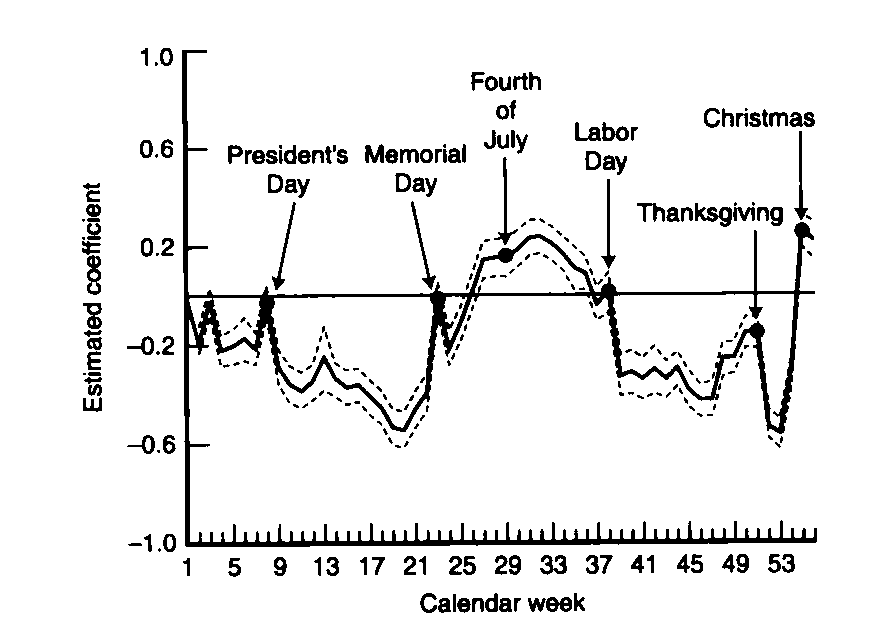
\includegraphics[width=\linewidth]{figures/ch07/einav_fig3_top.png}
\caption{With movie fixed effects}
\end{subfigure}\hfill
\begin{subfigure}[b]{0.49\textwidth}
\centering
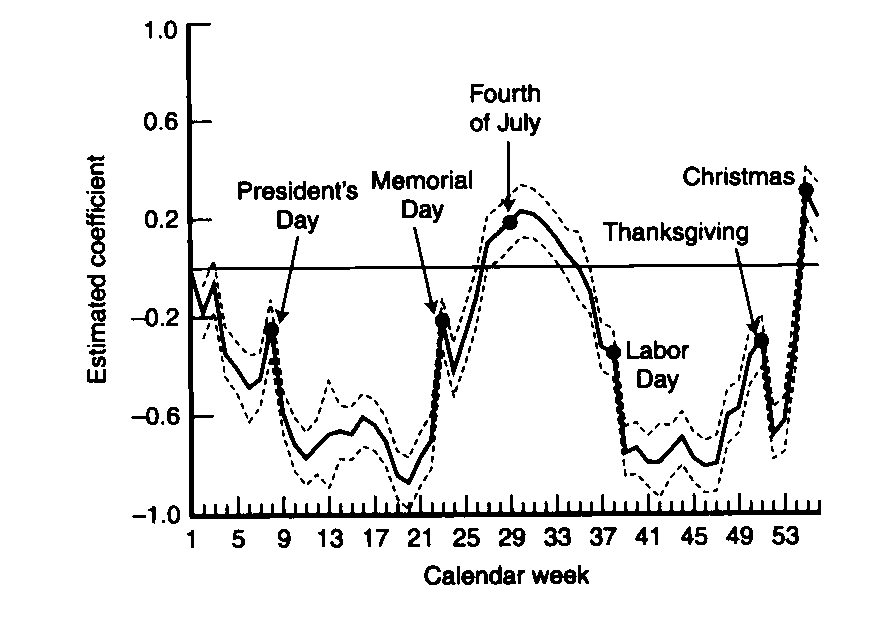
\includegraphics[width=\linewidth]{figures/ch07/einav_fig3_bottom.png}
\caption{Without movie fixed effects}
\end{subfigure}
\caption{Estimated week effects $\hat\tau_t$ by calendar week in the benchmark model of \citet{Einav2007}.
Panel (a) is the top panel and panel (b) the bottom panel of the original figure. Dashed lines mark two standard
errors. Source: \citet{Einav2007}, Figure 3.}
\label{fig:07-einav-seasonality}
\end{figure}

Underlying demand resembles revenue, high in summer and the holidays and low in spring and fall, but the
differences are informative (p.~138). Memorial Day, the Fourth of July and Thanksgiving, the big release weekends,
have high underlying demand, though less so relative to adjacent weeks than revenues suggest. Labor Day, when few
movies open, has much higher underlying demand than its revenue implies. Underlying demand is flat over the summer
and drops sharply after Labor Day, whereas revenues peak in early July and decline gradually, because the biggest
movies open early in the summer.

With $\lambda = 0.220$ and $\hat\sigma = 0.524$, Einav reports weekly revenue decay of 37 percent. For a movie too
small to move $D_t$, $\ln s_{jt}$ equals $\frac{\delta_{jt}}{1-\sigma}$ plus terms in $D_t$, so one more week
changes log share by $-\frac{0.220}{0.476} = -0.462$, and $1 - e^{-0.462} = 0.37$. Ten decay dummies give an almost
linear pattern. A linear time trend is not identified (footnote 19). If mean utility included $b\,t$, writing
$b\,t = b\,r_j + b(t - r_j)$ shows that it loads onto the movie effects, $\phi_j + b\,r_j$, and
onto the decay, $\lambda - b$. The movie effects, which show no trend, measure quality relative to an outside
good that may itself be changing.

\Cref{tab:07-einav-fe} projects the estimated movie effects on observables. Production cost, advertising and
Oscar recognition raise estimated quality, and restrictive ratings lower it. The adjusted $R^2$ is at most 0.387,
which Einav reads as the justification for fixed effects.

\begin{table}[htbp]
\centering
\caption{Projection of the estimated movie fixed effects on observables \citep[Table 3]{Einav2007}}
\label{tab:07-einav-fe}
\small
\begin{tabular}{lccc}
\toprule
Dependent variable: estimated movie effect $\hat\phi_j$ & (1) & (2) & (3) \\
\midrule
Log production cost & 0.215$^{**}$ (0.021) & 0.389$^{**}$ (0.021) & 0.384$^{**}$ (0.020) \\
Log advertising expenditure & 0.367$^{**}$ (0.019) & & \\
MPAA rating PG-13 & $-0.125^{**}$ (0.038) & $-0.135^{**}$ (0.043) & \\
MPAA rating R & $-0.154^{**}$ (0.039) & $-0.144^{**}$ (0.044) & \\
MPAA rating above R & $-0.442$ \phantom{$^{**}$}(0.365) & $-0.716^{*}$ \phantom{$^{*}$}(0.413) & \\
Genre comedy & $-0.052$ \phantom{$^{**}$}(0.035) & 0.029 \phantom{$^{**}$}(0.039) & \\
Genre drama & $-0.097^{**}$ (0.037) & $-0.021$ \phantom{$^{**}$}(0.040) & \\
Genre children & $-0.070$ \phantom{$^{**}$}(0.054) & $-0.037$ \phantom{$^{**}$}(0.060) & \\
Best picture nominee & 0.433$^{**}$ (0.081) & & \\
Best picture award & 0.467$^{**}$ (0.139) & & \\
Year fixed effects & yes & yes & no \\
$N$ & 1,542 & 1,603 & 1,603 \\
Adjusted $R^2$ & 0.387 & 0.208 & 0.193 \\
\bottomrule
\end{tabular}
\par\medskip
\parbox{\linewidth}{\footnotesize Notes: Standard errors in parentheses. $^{*}$ significant at the 10 percent
level, $^{**}$ at the 1 percent level. Omitted categories are rating PG and genre action. Blank cells are
variables not included. Samples are smaller than 1,956 because production cost and advertising are missing for
some movies. Source: \citet{Einav2007}, Table 3.}
\end{table}

\subsection{Robustness}\label{sec:07-einav-robust}

Predicted shares reproduce the observed seasonal pattern well, but the model underpredicts revenue in early summer
and the holidays and overpredicts it elsewhere (Figure 4, p.~139). Movies released in strong seasons decay more
slowly. Interacting decay with movie size, instrumented by production cost times decay, shows that better movies
decay more slowly and improves fit, but underlying seasonality barely moves. Letting decay vary by release season
gives $-0.194$ for holiday releases, $-0.206$, $-0.216$ and $-0.214$ for winter, spring and early summer, and
$-0.249$ and $-0.244$ for late summer and fall (pp.~139--140). Equality of the first four is not rejected, and
equality of the last two with the others is rejected. The summer week effects are unchanged.

Results are almost identical after dropping the first three weeks of each run, for movies with a full 10-week run
and for Friday releases (p.~140). Panel B of \cref{tab:07-einav-benchmark} shows faster decay in later
subperiods, consistent with wider openings, while underlying seasonality is stable. Alternative instruments, the
budget of competing movies, the number in the same genre, or the number released within a three-week or five-week
window, give similar results. The window counts address one source of endogeneity. Fewer movies may be shown in a week
when a strong movie is released. If distributors can move a release date by only a few weeks, counts over a window
around the week account for this response (footnote 20). Instruments
interacted with a measure of the movie's ex-ante size, such as production cost, are weaker. They give low estimates
of $\sigma$ and somewhat different results, but adding them to the main instruments leaves the reported results in
place (footnote 21). The nested logit ties expansion from more movies to expansion from better movies
through one parameter. \citet{AckerbergRysman2005} suggest adding the log number of products as a regressor, which
here is the instrument. Including it through functional form or with other instruments changes little
(pp.~140--141).

\subsection{Implications for release dates}\label{sec:07-einav-timing}

Set $\xi_{jt} = 0$ and write $Q_{kt} = \exp\big(\frac{\phi_k - \lambda(t-r_k)}{1-\sigma}\big)$ for the
decay-adjusted quality index and $C_t = \sum_{k \in \mathcal{J}_t} Q_{kt}$ for the \emph{competition effect}. Since
$D_t = \exp\big(\frac{\tau_t}{1-\sigma}\big)C_t$, dividing numerator and denominator of $s_{jt}$ by
$\exp\big(\frac{\tau_t}{1-\sigma}\big)$ gives
\begin{equation}\label{eq:07-einav-eq6}
s_{jt} = \frac{Q_{jt}}{C_t^{\sigma}}\,\Big[e^{-\tau_t} + C_t^{1-\sigma}\Big]^{-1}
\end{equation}
(Einav's equation (6)). The market-size term $e^{-\tau_t}$ is small when underlying demand is high. Competition
matters more as $\sigma$ rises, because movies then steal more from each other. With fixed prices and nearly zero
marginal cost, a price-taking distributor picks $r_j$ to maximize $\sum_{t=r_j}^{r_j+H}s_{jt}$ for a horizon $H$,
taking rivals' dates as given (pp.~141--142). Competition peaks at the start of the summer and at Christmas. Labor
Day combines high underlying demand with soft competition, and a small movie could double its revenue by opening
then instead of on Thanksgiving (p.~143). Large movies, Einav cautions, internalize their effect on competition.

If the industry could coordinate, with $n_w$ small divisible movies of quality index $e^{\frac{\bar\phi}{1-\sigma}}$
opening in week $w$, then $C_w^{1-\sigma} = n_w^{1-\sigma}e^{\bar\phi}$. Summing \eqref{eq:07-einav-eq6} over movies
gives the industry share $\frac{C_w^{1-\sigma}}{e^{-\tau_w} + C_w^{1-\sigma}}$, and the industry solves
\begin{equation}\label{eq:07-einav-eq7}
\max_{\{n_w\}}\ \sum_{w=1}^{W}\frac{n_w^{1-\sigma}e^{\bar\phi}}{e^{-\tau_w} + n_w^{1-\sigma}e^{\bar\phi}}
\quad\text{subject to}\quad \sum_{w=1}^{W} n_w = N,
\qquad
\frac{e^{-\tau_w}(1-\sigma)n_w^{-\sigma}e^{\bar\phi}}{\big(e^{-\tau_w} + n_w^{1-\sigma}e^{\bar\phi}\big)^2} = \mu
\end{equation}
(equations (7) and (8), with $\varepsilon$ in the paper for $\bar\phi$ and $\mu$ the Lagrange multiplier). The left side
of the first-order condition has a positive cross-partial in $\tau_w$ and $n_w$ at the estimates, so the optimum
puts more movies in high-demand weeks. The observed pattern yields a total industry share of 3.94 (observed:
3.92), and the optimum raises it only to 3.98, about 1 percent (p.~143). Quality is fixed in total, and with
$\sigma$ above 0.5 redistribution mostly moves revenue across movies.

\subsection{Interpretation and limitations}\label{sec:07-einav-assessment}

Einav attributes amplification to uniform ticket prices \citep{OrbachEinav2007}. The market can respond to high
demand only through the number and quality of movies (p.~144). He expects amplification in video rental, music
and books, and dampening where capacity constraints raise peak prices, as in tourism and airlines. The paper also
shows when a logit-type model suffices. There is no price coefficient, and the model is never asked for cross-price
substitution, the case anticipated by the remark in \cref{sec:07-iia}. The limitations follow from the identifying
assumptions. Decay must not depend on the release date, and the season-specific estimates show some dependence.
Underlying seasonality must be stable across years, the market is the population, and the mix of moviegoers is
constant over the year. A single $\sigma$ ties two kinds of expansion, and the release exercise treats
distributors as price takers. \citet{Einav2010} models the timing game as a sequential-move game with private
information. He finds release dates too clustered on holiday weekends, and that shifting some holiday releases by
a week or two would raise revenue.

\section{Case study: Hendel (1999), multiple discrete choice}\label{sec:07-hendel}

Every model so far has a consumer buy one unit of one product. \citet{Hendel1999} drops both restrictions for
business purchases of personal computers. We work mainly from the 1994 working paper \citep{Hendel1994}. Its pages
carry the prefix WP, and all equation and table numbers refer to it. Citations of the published article give its
own pages. The two versions may differ in specification and numbers.

\subsection{Question and motivating facts}\label{sec:07-hendel-question}

Hendel estimates PC demand by business establishments as an input to three questions (WP pp.~2--3). The first
is the ``computerization puzzle,'' the absence of measured productivity gains from computers in aggregate data.
The second is the gain from technical progress in components, and the third is quality adjustment in price
indices. \Cref{tab:07-hendel-freq}
reproduces Table I, the joint frequency of the number of PCs and the number of PC types held by 5,234
establishments that hold at least one PC. Only 1,369 hold a single PC and 2,367 a single type, while twelve hold
more than 2,000 units. Hendel concludes that multiple discreteness is the main feature of the data and that
aggregation misleads, since one firm buying 2,000 units differs from 2,000 firms buying one (WP p.~6).

\begin{table}[htbp]
\centering
\caption{Joint frequency of the number of PCs and the number of PC types held \citep[Table I]{Hendel1994}}
\label{tab:07-hendel-freq}
\small
\setlength{\tabcolsep}{4.5pt}
\begin{tabular}{lrrrrrrrrrr}
\toprule
 & \multicolumn{9}{c}{Number of PC types held} & \\
\cmidrule(lr){2-10}
Number of PCs & 1 & 2 & 3 & 4--6 & 7--9 & 10--19 & 20--49 & 50--99 & 100+ & Total \\
\midrule
1 & 1,369 & & & & & & & & & 1,369 \\
2 & 335 & 308 & & & & & & & & 643 \\
3--4 & 271 & 215 & 196 & & & & & & & 682 \\
5--6 & 123 & 99 & 129 & 29 & & & & & & 380 \\
7--10 & 104 & 111 & 152 & 52 & 7 & & & & & 426 \\
11--15 & 39 & 59 & 102 & 56 & 26 & & & & & 282 \\
16--35 & 68 & 84 & 154 & 99 & 65 & 8 & 2 & & & 480 \\
36--60 & 24 & 31 & 68 & 45 & 61 & 15 & 5 & & & 249 \\
61--100 & 12 & 12 & 51 & 39 & 47 & 16 & 8 & & & 185 \\
101--300 & 16 & 17 & 59 & 74 & 100 & 56 & 21 & 3 & & 346 \\
301--600 & 4 & 3 & 18 & 26 & 29 & 23 & 8 & 0 & 1 & 112 \\
601--1,000 & 2 & 0 & 3 & 8 & 8 & 11 & 6 & 1 & 0 & 39 \\
1,001--2,000 & 0 & 1 & 1 & 7 & 5 & 7 & 4 & 3 & 1 & 29 \\
2,000+ & 0 & 0 & 2 & 3 & 2 & 2 & 0 & 1 & 2 & 12 \\
\midrule
Total & 2,367 & 940 & 935 & 438 & 350 & 138 & 54 & 8 & 4 & 5,234 \\
\bottomrule
\end{tabular}
\par\medskip
\parbox{\linewidth}{\footnotesize Notes: Counts of establishments in the Comtec survey. Rows are bins of the total
number of PCs held and columns bins of the number of distinct PC types. Source: \citet{Hendel1994}, Table I.}
\end{table}

\subsection{The model}\label{sec:07-hendel-model}

We rename Hendel's symbols. The establishment is $i$ (his $f$), its tasks are $k = 1, \dots, K_i$ (his $j$ and
$J_f$), and PC types are $j = 1, \dots, J$ (his $i$). The curvature of task returns is $a$, where he writes $\alpha$,
which would clash with the price coefficient. The brand weight $W_{ijk}$ keeps his name and is unrelated to the weighting
matrix $W$.

Establishment $i$ with demographics $D_i$ has $K_i \sim \text{Poisson}(\lambda_i)$ potential tasks, with
$\lambda_i = g_0 + g_1\,emp_i + g_2\,soft_i$, where $emp_i$ is employment and $soft_i$ the number of software types
(WP equation (23)). Profit is additive across tasks (equation (4)), which rules out complementarities between
tasks. With $X_{ijk}$ units of type $j$ in task $k$ and rental prices $P_j$, the return on task $k$ is
\begin{equation}\label{eq:07-hendel-return}
\pi_{ik} = \Big(\sum_{j} W_{ijk}X_{ijk}\Big)^{a} S(D_i) - \sum_{j}P_jX_{ijk},
\qquad
W_{ijk} = \big(A_{ik}\cdot C_j\big)^{m(D_i)},
\qquad 0 < a < 1
\end{equation}
(equations (5) and (6)). The vector $C_j$ stacks a brand indicator and $j$'s observed attributes (MHz, memory, word
size). The random coefficients $A_{ik}$ hold perceptions of each brand's unobserved quality (reliability, service,
compatibility) and valuations of the attributes. Perceptions are normal with brand-specific means and a common
variance, and the MHz valuation is normal. The \emph{return shifter} is $S(D_i) = \varsigma_0 + (\varsigma_1 +
\varsigma_{1,rd}\,drd_i)emp_i$, where the paper writes $s_0$ and $s_1$ for our $\varsigma_0$ and $\varsigma_1$.
The taste for quality is $m(D_i) = m_0 + m_1 wh_i + m_{1,rd}\,drd_i$, with $wh_i$ the number of white-collar
workers and $drd_i$ an R\&D indicator (equations (24) and (25)). With no adjustment costs and a perfect resale market,
a PC costs its one-year rental price, the purchase price less next year's resale value. Lacking data on used prices,
Hendel computes the resale value from the 25 percent annual fall in quality-adjusted prices found by
\citet{BerndtGriliches1993}. An old machine costs a fraction $d_0$ of the new rental price (WP p.~24).

\casehead{One brand per task}
Brands enter a task through the index $E_{ik} = \sum_j W_{ijk}X_{ijk}$ of effective units, at linear cost. For any
$E_{ik}$,
\begin{equation*}
\sum_j P_jX_{ijk} = \sum_j \frac{P_j}{W_{ijk}}\,W_{ijk}X_{ijk} \ \ge\ \Big(\min_j\frac{P_j}{W_{ijk}}\Big)E_{ik},
\end{equation*}
with equality when only the type with the highest \emph{performance-to-price ratio} $\frac{W_{ijk}}{P_j}$ is used.
With continuous random coefficients ties have probability zero, so each task uses one brand (WP pp.~11 and 19).
Multiple brands per establishment come from multiple tasks.

\casehead{Units within a task}
Ignoring integer constraints, the first-order condition for type $j$ is $aW_{ijk}^{a}X^{a-1}S(D_i) = P_j$ (equation
(10)), so
\begin{equation}\label{eq:07-hendel-xstar}
X^*_{ijk} = \left(\frac{aW_{ijk}^{a}S(D_i)}{P_j}\right)^{\frac{1}{1-a}}
\end{equation}
(equation (11)). Using the first-order condition, cost equals $aW_{ijk}^{a}(X^*)^{a}S(D_i)$, so
\begin{equation*}
\pi^*_{ijk} = (1-a)\,W_{ijk}^{a}S(D_i)(X^*)^{a}
= (1-a)\,W_{ijk}^{a}S(D_i)\left(\frac{aW_{ijk}^{a}S(D_i)}{P_j}\right)^{\frac{a}{1-a}}
= (1-a)\,S(D_i)^{\frac{1}{1-a}}\left(\frac{aW_{ijk}}{P_j}\right)^{\frac{a}{1-a}}
\end{equation*}
(equation (12)), where $S$ has exponent $1 + \frac{a}{1-a} = \frac{1}{1-a}$ and $W$ has exponent $a + \frac{a^2}{1-a}
= \frac{a}{1-a}$. The maximized return rises with $\frac{W_{ijk}}{P_j}$. With integer units the best brand can
change, for example when its optimum is 3.5 units (WP p.~12). Returns are concave in $X$, so the integer optimum
is $\lfloor X^*\rfloor$ or $\lceil X^*\rceil$, and the algorithm compares these $2J$ candidates (WP p.~20). When
$X^* < 1$ the lower candidate is zero, meaning no PC for the task.

\casehead{Horizontal and vertical differentiation}
Brand perceptions that differ across establishments create horizontal differentiation. The exponent $m(D_i)$
creates vertical differentiation. If buyers agree on a quality index $q$ facing a convex price schedule $P(q)$,
equation (12) has them maximize $\frac{q^m}{P(q)}$, whose first-order condition is $m = \frac{P'(q^*)q^*}{P(q^*)}$
(WP Appendix 2). When the price elasticity of quality rises with $q$, as Hendel argues from convexity, buyers with
higher $m$ choose better machines.\footnote{The main text of the working paper writes this condition with $W$ in
place of the index (equation (13)). We follow its Appendix 2.} A multiplicative taste would not work, since scaling
all $W$ leaves the ranking of $\frac{W}{P}$ unchanged. In Bresnahan's single-unit vertical model it works because
buyers purchase one unit (WP endnote 4). By \eqref{eq:07-hendel-xstar}, $S(D_i)$ moves the number of units but,
entering every brand's return through the factor $S^{\frac{1}{1-a}}$, leaves the brand choice unchanged. The taste
$m(D_i)$ moves the brand choice. Hendel argues that these distinct roles identify the two functions (WP p.~13).

\subsection{Estimation}\label{sec:07-hendel-estimation}

Expected purchases average the task-level choices over tasks and random coefficients,
\begin{equation}\label{eq:07-hendel-expected}
X^e_i(D_i, \theta) = \sum_{K=0}^{\infty}\Pr(K_i = K \mid D_i)\sum_{k=1}^{K}\int X^*_{ik}(D_i, A, \theta)\,
\mu(\dd A \mid D_i, \theta)
\end{equation}
(WP equation (15)), where $X^*_{ik}$ is the $J$-vector of task purchases and $\mu$ the normal distribution of the
coefficients. The prediction error $e_i(\theta) = X^e_i(D_i, \theta) - X_i$ has mean zero given $D_i$ at the true
$\theta$, so $G(\theta) = \E[T(D_i)\otimes e_i(\theta)] = 0$ for any function $T$ of demographics (equations (16)
to (18)). Hendel minimizes a quadratic form in the sample analogue over the $F$ establishments, $G_F(\theta) =
\frac{1}{F}\sum_{i=1}^F T(D_i)
\otimes(X^e_i(\theta) - X_i)$ with the efficient weighting matrix \citep{Hansen1982}. Demographics are valid
instruments by construction, since predictions condition on them.

The integral is simulated \citep{McFadden1989,PakesPollard1989}. For each establishment and simulation round,
Hendel draws a number of tasks and the coefficients of each task, and solves each integer problem. The moments are
linear in simulated purchases, so the estimator is consistent as $F$ grows with the number of draws fixed (WP
pp.~18--19). A device keeps draws fixed while $\lambda_i$ changes in the search (WP Appendix 3). Let $E_1, E_2,
\dots$ be i.i.d.\ exponential with mean one and $Y_k = \sum_{l\le k}E_l$, which is gamma with shape $k$. Integrating
by parts $k-1$ times,
\begin{equation*}
\Pr(Y_k < \lambda) = 1 - \sum_{l=0}^{k-1}\frac{e^{-\lambda}\lambda^{l}}{l!} = \Pr(N \ge k),
\qquad N \sim \text{Poisson}(\lambda),
\end{equation*}
so the number of partial sums below $\lambda$ is Poisson with mean $\lambda$. Holding the exponential draws fixed
holds the randomness constant across trial parameters. The simulated objective is then a step function, a case
covered by \citet{PakesPollard1989}. Standard errors from numerical derivatives proved sensitive to the step, so
Hendel averages over three steps and also reports a bootstrap (WP endnote 12).

Hendel argues that the joint distribution of units and types in \cref{tab:07-hendel-freq} identifies the task
process (WP p.~20). We add an observation on the moments he uses, which are brand-level purchase totals interacted
with demographics (45 moments for 15 types). Tasks are i.i.d.\ given $D_i$ and independent of $K_i$, so Wald's
identity gives
\begin{equation*}
\E[X_i \mid D_i] = \lambda_i\,\E\big[X^*_{ik}(D_i, A_{ik}, \theta) \mid D_i\big].
\end{equation*}
These moments see the task process only through $\lambda_i$. It multiplies per-task purchases, which scale with
$S(D_i)^{\frac{1}{1-a}}$ apart from integer effects. Tasks and the return shifter are therefore separated through
the integer constraint and through variables that enter only one function, $soft_i$ in $\lambda_i$. Moments on the
number of types held would use \cref{tab:07-hendel-freq} more directly.

\subsection{Data and results}\label{sec:07-hendel-results}

Prices and attributes of microcomputers from 1976 to 1989 come from \citet{BerndtGriliches1993}, who collected them
from magazine advertisements (WP pp.~21--23). Holdings come from the Comtec survey of about 8,000 representative
non-farm establishments in 1984 and 1988, stratified by size and sector with extrapolation weights. Large
establishments are oversampled. Unweighted means are 241.55 employees and 35.05 PCs, and weighted means 15.49 and
1.96 (Tables II and III). Estimation uses 123 randomly chosen establishments out of 546 in banking (finance,
insurance and real estate), with more than 1,000 purchases. The choice set has 15 types (WP Appendix 4). They are four IBM models (8086, 8088, 286,
386), three Apple models, two each from Zenith and Compaq, three clones and the AT\&T 8086. The IBM 286 leads with a price of \$2,700 and a 37.3 percent share of 1986--1988 sales.

\begin{table}[htbp]
\centering
\caption{Parameter estimates for the banking sector \citep[Table V]{Hendel1994}}
\label{tab:07-hendel-params}
\small
\begin{tabular}{llccc}
\toprule
Parameter & Meaning & Estimate & Numerical s.d. & Bootstrap s.d. \\
\midrule
$\varsigma_0$ & Intercept of $S(D_i)$ & 0.61 & n.a. & 0.19 \\
$\varsigma_1$ & Slope of $S(D_i)$ in employment & 0.47 & 0.18 & 0.06 \\
$m_1$ & Slope of $m(D_i)$ in white-collar workers & $6\times 10^{-4}$ & $1.3\times 10^{-4}$ & $10^{-5}$ \\
$a$ & Task-return exponent & 0.29 & 0.03 & 0.04 \\
$\Var(A_j)$ & Variance of brand perceptions & 3.50 & 0.55 & 0.92 \\
$A_M$ & Mean valuation of MHz & 0.89 & 0.24 & 0.16 \\
$\Var(A_M)$ & Variance of MHz valuation & 1.48 & 0.78 & 0.23 \\
$A_R$ & Valuation of memory (RAM) & 0.53 & 0.11 & 0.06 \\
$A_{B16}$ & 16-bit dummy & 0.78 & 0.87$^{b}$ & n.a. \\
$A_{B32}$ & 32-bit dummy & 1.17 & 2.93$^{b}$ & n.a. \\
$g_1$ & Task mean, slope in employment & 2.42 & 1.34$^{a}$ & 0.32 \\
$g_2$ & Task mean, slope in software types & 0.78 & 0.18 & 0.10 \\
$d_0$ & Relative cost of keeping an old PC & 0.79 & 0.09 & 0.19 \\
\midrule
\multicolumn{5}{l}{Objective function $G_F(\theta) = 405$, with 45 moments and 25 parameters} \\
\bottomrule
\end{tabular}
\par\medskip
\parbox{\linewidth}{\footnotesize Notes: Simulated method of moments, 123 banking establishments. Numerical
standard deviations average numerical derivatives over three step sizes. Bootstrap standard deviations come from
50 bootstrap rounds. $^{a}$ significant at the 10 percent level, $^{b}$ not significant (the paper's markers).
The intercepts $g_0$ and $m_0$ are fixed at 0.1 and 1.0. The paper writes $\alpha_0$ (A$_0$ in the table) for
the exponent we call $a$. Brand-specific mean perceptions are in the paper's Table VII. Source:
\citet{Hendel1994}, Table V.}
\end{table}

\Cref{tab:07-hendel-params} reproduces Table V. The curvature $a = 0.29$ lies in $(0, 1)$, as interior solutions
require. Larger establishments buy more PCs ($\varsigma_1$), and establishments with more white-collar workers prefer
higher quality ($m_1$). The significant variance of brand perceptions, 3.50, means buyers perceive the same machine
differently, a horizontal dimension. MHz has a significant mean and variance, memory a significant coefficient,
and users trade 1.6K of expandable memory for one more MHz. Word size is insignificant. The task process rises
with size and software variety. Keeping an old PC costs $d_0 = 0.79$ of a new one, with a $t$-statistic of 2.29
for $1 - d_0$, and the implied 20 percent gap matches new and used prices (WP pp.~26--28). Mean perceptions
(Table VII) average 54.1 for IBM, 40.9 for Compaq, 28.5 for Apple, 20.1 for clones, 16.5 for Zenith and 2.9 for
AT\&T. The objective, 405, is treated as $\chi^2$ with 20 degrees of freedom. Hendel quotes a 5 percent cutoff of
30 (the exact value is 31.4), so the model is rejected (WP p.~26).

A separate estimation adds the R\&D and education sectors to banking and reports sector effects in Table VI (WP
p.~25). It omits the word-size dummies of Table V, so its estimates are not directly comparable with those of
\cref{tab:07-hendel-params}.
\Cref{tab:07-hendel-sectors} reproduces it. The extra employment slope of $S(D_i)$ for R\&D establishments,
$\varsigma_{1,rd} = 0.69$, is significant, so their purchases are more sensitive to size. Hendel expects this from
complementarity between labor and PCs in R\&D, and it fits their higher ratio of PCs to employees (WP Table IV). The
R\&D shift in the taste for quality, $m_{1,rd} = 0.70$ with a standard deviation of 7.00, is insignificant. There is
no vertical dimension tied to the sector, which fits the observation that R\&D establishments do not hold more
valuable PCs than banks. The education sector's extra employment slope is also insignificant. Its extra taste for
Apple machines, 4.20, is ``borderline significant'' in Hendel's words, with a ratio to its standard deviation of 1.39.
He equates it to about 4 MHz, so a school values an Apple like a non-Apple machine with 4 more MHz (WP pp.~26--28).
The working paper's text calls it Table VI on WP pp.~25--27 and Table VII on WP p.~28.

\begin{table}[htbp]
\centering
\caption{Sector effects when R\&D and education establishments are added \citep[Table VI]{Hendel1994}}
\label{tab:07-hendel-sectors}
\small
\begin{tabular}{llcc}
\toprule
Parameter & Meaning & Estimate & Std.\ dev. \\
\midrule
$\varsigma_{1,rd}$ & Extra employment slope of $S(D_i)$, R\&D sector & 0.69 & 0.11 \\
$\varsigma_{1,ed}$ & Extra employment slope of $S(D_i)$, education sector & 1.00 & 3.33 \\
$m_{1,rd}$ & R\&D dummy in $m(D_i)$, vertical by sector & 0.70 & 7.00 \\
$A_{\text{Apple}}$ & Extra valuation of Apple, education sector & 4.20 & 3.02 \\
\bottomrule
\end{tabular}
\par\medskip
\parbox{\linewidth}{\footnotesize Notes: Simulated method of moments on banking, R\&D and education
establishments, estimated separately from \cref{tab:07-hendel-params} and without the word-size dummies. The paper
writes $s_{1RD}$, $s_{1ED}$ and $M_{1RD}$ for our $\varsigma_{1,rd}$, $\varsigma_{1,ed}$ and $m_{1,rd}$.
Source: \citet{Hendel1994}, Table VI (WP p.~47).}
\end{table}

Elasticities come from numerically differentiating simulated demand (Table VIII). The text implies that the
table's rows index the product whose price changes and its columns the product whose demand responds. Only this
reading matches three statements of the text (WP p.~31), which calls the table Table VII. The IBM 286 and IBM 386 are
each other's closest substitutes, and the Zenith 8088 responds most to the IBM 8088 price. The Apple 68020 responds
strongly to the IBM 286 price, a machine in a similar price and attribute range, with a cross elasticity of 38.29.
Own elasticities are printed as negative numbers, from
$-0.13$ (Apple 68000) and $-0.93$ (IBM 8086) to $-7.9$ (Apple 68020). Two below one in absolute value sit uneasily
with Nash pricing.

\subsection{Welfare and implications}\label{sec:07-hendel-welfare}

Hendel values PCs with Hotelling's lemma. Let $\Pi_i(\boldsymbol P)$ be maximized profit from PCs at rental prices
$\boldsymbol P$, relative to the outside option of no PCs, so $\Pi_i(\infty) = 0$ and $\frac{\partial
\Pi_i}{\partial P_j} = -X_{ij}(\boldsymbol P)$. Integrating from the 1988 prices $\boldsymbol P^0$,
\begin{equation*}
\Pi_i(\boldsymbol P^0) - \Pi_i(\infty) = \int_{\boldsymbol P^0}^{\infty} X_i(\boldsymbol P)\cdot\dd\boldsymbol P,
\end{equation*}
the area under the input demand curve. In practice he evaluates the estimated profit function at predicted
behavior and extrapolates with survey weights (WP p.~29). Banking held 729,922 PCs in 1988 and earned about \$1.2
billion from them, about \$1,300 per PC per year against an average annual rental price of
\$1,443.\footnote{Dividing \$1.2 billion by 729,922 gives about \$1,640 per PC. The working paper does not explain
the difference.} The ratio, about 90 percent, is the reported return on investment, an upper bound because
training costs are omitted. Hendel puts the gain at 3.5 percent of the sector's 1988 profits of \$41.8
billion.\footnote{The ratio of the reported figures, $\frac{1.2}{41.8}$, is about 2.9 percent.} A simulated
standard deviation is about \$0.2 billion (WP endnote 14). Treating each type held as one task gives a lower
bound of \$956.25 million (WP p.~31). Bresnahan's estimate for mainframes in 1972 is a surplus of \$225 to \$417
million on \$68 million of spending, in 1989 dollars \citep{Bresnahan1986}. The profit function is cardinal, anchored in money by
PC prices, and the gain is relative to minicomputers, mainframes or no equipment (WP p.~30).

Assuming static Nash pricing, the IBM 386, an \$8,000 machine, has marginal revenue of \$6,350, an implied markup
of \$1,650 (WP pp.~31--32). Making all microprocessors 10 percent faster at unchanged prices raises end-user
surplus by 4 percent, ignoring supplier responses. A hedonic price elasticity with respect to MHz of 0.458
\citep{BerndtGriliches1993} gives 4.58 percent, so hedonic prices are close to marginal benefits here.

\subsection{Limitations, relation to logit, and contribution}\label{sec:07-hendel-assessment}

The model rules out complementarities across tasks, and one brand per task holds by construction, so two brands
in one job count as two tasks (WP p.~19). Tasks are unobserved, and mapping software types into tasks failed (WP
endnote 8). Durability enters only through a rental price. The intercepts $g_0$ and $m_0$ are fixed, the sample is
123 establishments in one sector, and the overidentification test rejects. Prices vary only across 15 types in one
cross section, and brand means absorb quality. The price response therefore rests largely on the structure of the
task problem, in which $a$ governs both scale and price response.

The working paper has normal random coefficients and no extreme value shock, so it is not a logit. The published
article has no extreme value shock either. Its random coefficients on all brand dummies and on MHz are normal, and
the number of potential tasks is Poisson \citep[p.~437]{Hendel1999}. A logit reading is still instructive. By WP equation (12), $\ln\pi^*_{ijk} = c_{ik} + \frac{a}{1-a}[m(D_i)\ln(A_{ik}\cdot C_j) - \ln
P_j]$, where $c_{ik}$ does not depend on the brand. Suppose the brand-specific part of $m(D_i)\ln(A_{ik}\cdot C_j)$ had an
additive i.i.d.\ type-I extreme value component. Ignoring integer constraints, each task's brand choice would then be
a logit in $\ln W - \ln P$ with coefficient $\frac{a}{1-a}$. With the random MHz coefficient it would
be a mixed logit, and establishment demand a Poisson mixture of such choices. This interpretation is ours. Hendel
notes that his framework allows any distributional assumption, not just extreme value
\citep[pp.~424--425]{Hendel1999}.

Hendel made multiple discreteness an estimable demand structure with microfoundations. Discrete-continuous models
allow one discrete choice and a continuous quantity \citep{DubinMcFadden1984,Hanemann1984}, and
\citet{ManskiSherman1980} allow up to two cars per household. Tasks allow any number of units of any brands while
each task stays a simple discrete choice. \citet{Dube2004} applies the idea to soft drinks, and
\citet{Gentzkow2007} allows goods to be complements in a multiple-choice model of newspapers (\cref{ch:newgoods}).

\section{The limits of logit and the road to random coefficients}\label{sec:07-limits}

The logit and nested logit are cheap, transparent and linear after inversion, and \citet{Einav2007} shows that they
serve when elasticities are not the object. When elasticities, markups or substitution are the object, their
restrictions bind. \citet{BerryLevinsohnPakes1995} estimate both a logit and a random-coefficients model on the
same automobile data, which makes the comparison clean.

\subsection{Own-price elasticities rise with price}\label{sec:07-limits-own}

The logit own elasticity is $\varepsilon_j = \alpha p_j(1 - s_j) \approx \alpha p_j$, since each car's share of
all households is very small. BLP's IV logit gives $\hat\alpha = 0.216$ (0.123), with prices in thousands of 1983
dollars (\cref{tab:07-blp-logit}). For 13 models of 1990, BLP's Table V reports the random-coefficients
elasticities, which \cref{tab:08-blp-attr} reproduces and \cref{fig:08-blp-ownelas} plots against the logit benchmark.
The IV logit implies elasticities from about 1.1 for the Mazda 323 (\$5,049) to about 8.1 for the BMW 735i
(\$37,490). The random-coefficients model reverses the ranking. Its elasticities lie between 6.0 and 6.6 for the four
cheapest models and fall to 3.5 for the BMW and 3.1 for the Lexus LS400. The most elastic demands are in the crowded
compact and subcompact segments, with the Buick Century (6.8) as an exception (p.~879).

The logit pattern follows from a common price coefficient. Buyers of expensive cars are assumed to be as sensitive
to a dollar as buyers of cheap ones, so the elasticity, price coefficient times price, is largest for expensive
cars. A referee suggested to BLP that $\ln p$ in place of $p$ would give more reasonable markups. It did, but
substitution patterns remained ``quite unreasonable'' (p.~874, footnote 26).

\subsection{Substitution goes to the outside good}\label{sec:07-limits-outside}

The diversion ratio to the outside good, $D_{j0} = -\frac{\partial s_0}{\partial p_j}\big(\frac{\partial
s_j}{\partial p_j}\big)^{-1}$, is the share of those leaving $j$ after a small price rise who buy nothing. In the
logit, $\frac{\partial s_0}{\partial p_j} = \alpha s_js_0$ and $\frac{\partial s_j}{\partial p_j} = -\alpha
s_j(1-s_j)$, so $D_{j0} = \frac{s_0}{1-s_j}$. Most households buy no new car in a year, so $s_0$ is near 0.9.
BLP's Table VII, reproduced in \cref{tab:08-blp-outside}, reports this diversion ratio for the same 13 models. The
logit column lies between 90.46 and 90.88 percent, and BLP state that it is $\frac{s_0}{1-s_j}$. The
random-coefficients column generally falls with price, from 27.1 percent for the Mazda 323 and 28.0 for the Ford Escort to 10.1
for the Lexus LS400 and the BMW 735i. Buyers of these luxury cars who react to a price rise mostly
switch to other luxury cars. BLP still find these numbers ``a bit large'' (p.~881).

A logit therefore overstates how much industry demand falls when prices rise, and it understates competition
between close substitutes, because diversion is proportional to shares whatever the similarity of products. BLP's
random-coefficients semi-elasticities make the Lexus the closest substitute to the BMW 735i, the Cadillac to the
Lincoln, and the Accord to the Taurus (p.~881). In a logit every car's closest substitute is the best seller. For
merger analysis, which turns on diversion between the merging products (\cref{ch:mergers}), this is the wrong
pattern.

\subsection{Markups are nearly equal}\label{sec:07-limits-markups}

With logit demand a firm sets the same dollar markup $\frac{1}{\alpha(1 - S_f)}$ on all its products
(\cref{prop:07-logit-multi}), never below $\frac{1}{\alpha}$. \Cref{sec:07-conduct} showed what this implies for
BLP's IV logit. Markups lie between \$4,630 (BMW) and \$4,805 (Chevy Cavalier), highest for GM, which makes the most
models, and ``quite counter-intuitively'' lowest for BMW (p.~874). The floor $\frac{1}{0.216} = 4.63$ thousand
dollars is BMW's markup. Percentage markups then fall steeply with price. By our computation the implied Lerner
indices are $\frac{4.805}{5.797} = 0.83$ for the Cavalier and $\frac{4.63}{37.49} = 0.12$ for the BMW, and 83 percent
is implausible for an economy car. The same rigidity affects conduct counterfactuals. With logit demand, joint
ownership of 25 cereal brands raises Nevo's median margin only to 41.9 percent, against 72.6 percent in his full
model (\cref{tab:07-nevo-margins,tab:08-nevo-margins}, \citealp{Nevo2001}). The logit spreads substitution evenly across brands and the
outside good.

\subsection{Too many characteristics}\label{sec:07-limits-epsilon}

Each new product brings its own $\epsilon_{ij}$ and a set of consumers who like it most, even if it is identical
or inferior to an existing product. The red and blue buses of \cref{sec:07-iia} are the standard example. Three biases follow. A
clone of product $j$ raises consumer surplus by $\frac{1}{\alpha}\ln(1 + s_j)$, and with $J$ identical products
expected maximum utility grows like $\ln J$ without bound (\cref{sec:07-welfare-apps}, \cref{fig:07-clones}).
Logit valuations of new goods are therefore biased upward (\cref{ch:newgoods}). Markups never vanish: with $J$ symmetric
single-product firms, each share $s = \frac{e^{\delta - \alpha p}}{1 + Je^{\delta - \alpha p}}$ goes to zero as $J
\to \infty$, so the markup $\frac{1}{\alpha(1-s)}$ converges to $\frac{1}{\alpha} > 0$ however crowded the market.
In the mirror image, every product has a positive predicted share, so products with zero sales cannot be used
(\cref{sec:07-market-size}, \citealp{GandhiLuShi2023}).

There are four responses. \citet{AckerbergRysman2005} make the role of the logit shock depend on the number of
products, which \citet{Einav2007} describes as adding the log number of products as a regressor. Nesting tempers
the problem within nests, since a clone in the same nest adds little as $\sigma \to 1$. The pure characteristics
model of \citet{BerryPakes2007} drops the shock, at the cost of shares that are not smooth in $\boldsymbol\delta$
and an inversion that is no longer a contraction. The hedonic approach of \citet{BajariBenkard2005} recovers each
consumer's tastes from the gradient of a hedonic price function and needs a dense product space.
\Cref{ch:discrete,ch:blp} develop these models.

\subsection{Heterogeneity is the cure}\label{sec:07-limits-cure}

By \cref{rem:07-berry-iid}, these restrictions come from the i.i.d. additive structure, so changing the distribution
of the shock does not remove them. Heterogeneity in tastes that is correlated across similar products does. With
$u_{ij} = x_j\beta_i - \alpha_ip_j + \xi_j + \epsilon_{ij}$, tastes distributed across consumers, and $s_{ij}$ the
logit probability of consumer $i$, shares are $s_j = \int s_{ij}\,\dd F(i)$ and
\begin{equation*}
\frac{\partial s_j}{\partial p_k} = \int \alpha_i s_{ij}s_{ik}\,\dd F(i) \quad (k \ne j),
\qquad
\frac{\partial s_j}{\partial p_j} = -\int \alpha_i s_{ij}(1 - s_{ij})\,\dd F(i).
\end{equation*}
Cross effects are large when the same consumers are likely to buy both products, that is, when the products are
similar in the dimensions over which tastes vary. The own elasticity can fall with price if buyers of expensive
products have low $\alpha_i$. Diversion to the outside good, $\int\alpha_i s_{ij}s_{i0}\,\dd F(i)$ divided by
$\int\alpha_i s_{ij}(1-s_{ij})\,\dd F(i)$, is small for products whose buyers rarely choose the outside good. The
nested logit is the special case with random coefficients on nest dummies (\cref{sec:07-berry-examples}).
\Cref{tab:07-model-comparison} summarizes, and \cref{ch:blp} develops the general model.

\begin{table}[htbp]
\centering
\caption{What logit, nested logit, and random-coefficients logit deliver}
\label{tab:07-model-comparison}
\small
\renewcommand{\arraystretch}{1.25}
\begin{tabularx}{\linewidth}{>{\raggedright\arraybackslash}p{0.2\linewidth}
  >{\raggedright\arraybackslash}X >{\raggedright\arraybackslash}X >{\raggedright\arraybackslash}X}
\toprule
 & Logit & Nested logit & Random-coefficients logit \\
\midrule
Shares & Closed form & Closed form & Integral, simulated \\
Inversion & $\ln s_j - \ln s_0$ & $\ln s_j - \sigma\ln s_{j\mid g} - \ln s_0$ & Numerical contraction \\
Estimation & Linear IV & Linear IV, two endogenous regressors & Nonlinear GMM with nested inversion \\
Substitution & Proportional to shares (IIA) & Proportional to shares within and across nests, more within the
  nest. IIA holds only within a nest &
  Toward products with similar characteristics \\
Own elasticity & $\alpha p_j(1-s_j)$, rises with price & Rises with price & Can fall with price \\
Diversion to outside good & $\frac{s_0}{1-s_j}$ & $\frac{(1-\sigma)s_0}{1 - \sigma s_{j\mid g} - (1-\sigma)s_j}$ &
  Depends on who buys $j$ \\
Multi-product markups & Equal within firm & Equal within firm and nest & Vary by product \\
Main inputs & Shares, prices, instruments & Plus nest assignment and instruments for $s_{j\mid g}$ &
  Plus instruments for the taste dispersion, ideally demographics or micro data \\
\bottomrule
\end{tabularx}
\par\medskip
\parbox{\linewidth}{\footnotesize Notes: Single-market formulas with the outside good normalized to zero mean
utility. Nested-logit entries are derived in \cref{sec:07-nested}, and random-coefficients entries in
\cref{ch:blp}.}
\end{table}

The logit and the one-nest nested logit remain useful first looks and robustness checks, and they are adequate
when the question does not turn on substitution patterns. Einav's seasonality decomposition is such a question.
Merger simulation, markup measurement and the valuation of new goods are not, and for those the
random-coefficients model of \cref{ch:blp} is the starting point.
